%
\section{Signals \& Slots}
\label{ref:soft-signal-slot}
In the project extensive use was made of the Signal and Slot mechanism, in order
 to allow communication between the objects in the code. Signals and slots are
used for communication between objects. The signals and slots mechanism is a
central feature of Qt and probably the part that differs most from the features
provided by other frameworks. Signals and slots are made possible by Qt’s
meta-object system.\cite{Qt:signal-slot}

\subsection{Introduction}
\label{ssec:soft-intro}
In GUI programming, when we change one widget, we often want another widget to
be notified. More generally, we want objects of any kind to be able to
communicate with one another.
%
Other tool kits achieve this kind of communication using callbacks. A callback is
a pointer to a function, so if you want a processing function to notify you
about some event you pass a pointer to another function (the callback) to the
processing function.\linebreak The processing function then calls the callback when
appropriate. While successful frameworks using this method do exist, callbacks
can be unintuitive and may suffer from problems in ensuring the type-correctness
of callback arguments.\cite{Qt:signal-slot}

\subsection{Signals and Slots}
\label{ssec:soft-sig-solt-detail}
In Qt, we have an alternative to the callback technique: We use signals and
slots. A signal is emitted when a particular event occurs. Qt's widgets have
many predefined signals, but we can always subclass widgets to add our own
signals to them. A slot is a function that is called in response to a particular
signal. Qt's widgets have many pre-defined slots, but it is common practice to
subclass widgets and add your own slots so that you can handle the signals that
you are interested in.\hfill \break
%
%
\begin{figure}[htb]
	\centering
	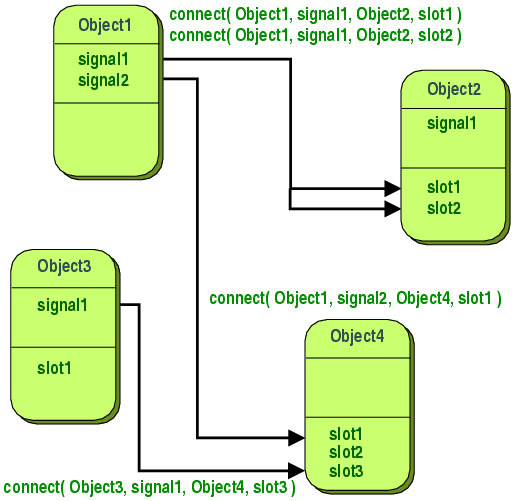
\includegraphics[width=0.65\textwidth]{abstract-connections.jpg}
	\captionsource{Signal and Slot scheme.}{
	\href{https://doc.qt.io/qt-5/signalsandslots.html}{https://doc.qt.io/qt-5/signalsandslots.html}}
	\label{fig:software-signal-slots-scheme}
\end{figure}
%
\newline The signals and slots mechanism is type safe: The signature of a signal must
match the signature of the receiving slot. (In fact a slot may have a shorter
signature than the signal it receives because it can ignore extra arguments.)
Since the signatures are compatible, the compiler can help us detect type
mismatches when using the function pointer-based syntax. The string-based
\textbf{SIGNAL} and \textbf{SLOT} syntax will detect type mismatches at runtime.
Signals and slots are loosely coupled: A class which emits a signal neither
knows nor cares which slots receive the signal. Qt's signals and slots mechanism
ensures that if you connect a signal to a slot, the slot will be called with the
signal's parameters at the right time. Signals and slots can take any number of
arguments of any type. They are completely type safe.
%
All classes that inherit from \texttt{QObject} or one of its subclasses (e.g.,
\texttt{QWidget}) can contain signals and slots. Signals are emitted by objects
when they change their state in a way that may be interesting to other objects.
This is all the object does to communicate. It does not know or care whether
anything is receiving the signals it emits. This is true information
encapsulation, and ensures that the object can be used as a software component.
%
Slots can be used for receiving signals, but they are also normal member
functions. Just as an object does not know if anything receives its signals, a
slot does not know if it has any signals connected to it. This ensures that
truly independent components can be created with Qt.
%
You can connect as many signals as you want to a single slot, and a signal can
be connected to as many slots as you need. It is even possible to connect a
signal directly to another signal. (This will emit the second signal immediately
whenever the first is emitted.)
%
Together, signals and slots make up a powerful component programming mechanism.\cite{Qt:signal-slot}

\subsection{Signals}
\label{ssec:soft-signal}
Signals are emitted by an object when its internal state has changed in some way
that might be interesting to the object's client or owner. Signals are public
access functions and can be emitted from anywhere, but we recommend to only emit
them from the class that defines the signal and its subclasses.
%
When a signal is emitted, the slots connected to it are usually executed
immediately, just like a normal function call. When this happens, the signals
and slots mechanism is totally independent of any GUI event loop. Execution of
the code following the emit statement will occur once all slots have returned.
The situation is slightly different when using queued connections; in such a
case, the code following the \textbf{\texttt{emit}} keyword will continue
immediately, and the slots will be executed later.
%
If several slots are connected to one signal, the slots will be executed one
after the other, in the order they have been connected, when the signal is
emitted.
%
Signals are automatically generated by the \emph{moc} and must not be implemented in
the \texttt{.cpp} file. They can never have return types (i.e. use void).\cite{Qt:signal-slot}

\subsection{Slots}
\label{ssec:soft-slots}
A slot is called when a signal connected to it is emitted. Slots are normal C++
functions and for this reason can be called normal; their only special feature
is that signals can be connected to them.
%
Since slots are normal member functions, they follow the normal C++ rules when
called directly. However, as slots, they can be invoked by any component,
regardless of its access level, via a signal-slot connection. This means that a
signal emitted from an instance of an arbitrary class can cause a private slot
to be invoked in an instance of an unrelated class.
%
Compared to callbacks, signals and slots are slightly slower because of the
increased flexibility they provide, although the difference for real
applications is insignificant. In general, emitting a signal that is connected
to some slots, is approximately ten times slower than calling the receivers
directly, with non-virtual function calls. This is the overhead required to
locate the connection object, to safely iterate over all connections (i.e.
checking that subsequent receivers have not been destroyed during the emission),
and to marshall any parameters in a generic fashion. 
While ten non-virtual function calls may sound like a lot, it's much less
overhead than any \texttt{new} or \texttt{delete} operation, for example. As
soon as you perform a string, vector or list operation that behind the scene
requires \texttt{new} or \texttt{delete}, the signals and slots overhead is only
responsible for a very small proportion of the complete function call costs. The
same is true whenever you do a system call in a slot; or indirectly call more
than ten functions. 
The simplicity and flexibility of the signals and slots mechanism is well worth
the overhead, which your users won't even notice.\cite{Qt:signal-slot}
